\chapter{Marco de referencia}

\section{Marco teórico}
\subsection{Sistema fotovoltaico}
Es el conjunto de equipos eléctricos y electrónicos que producen energía eléctrica a partir de la radiación solar. El principal componente de este sistema es el módulo fotovoltaico, a su vez compuesto por celdas capaces de transformar la energía luminosa incidente en energía eléctrica de corriente continua \cite{M1}. Dicho sistema cuenta con equipos y/o dispositivos complementarios dependiendo de la aplicación a la que esté destinado.\\

De acuerdo con O. Perpiñán Lamiguerio en \cite{M1}, un sistema fotovoltaico puede clasificarse en tres grandes grupos:

\begin{itemize}
	\item \textit{Conectados a la red}: Tienen la función de producir energía eléctrica en condiciones adecuadas para poder ser inyectada en la red convencional, por lo que no necesitan incorporar equipos de acumulación de energía; por otro lado, requieren del uso de un equipo inversor que adecúe la potencia producida por el generador fotovoltaico a las condiciones de la red convencional.
	\item \textit{Autónomos}: Su denominador común es la necesidad de satisfacer una demanda energética determinada. Por esta razón, prácticamente todos los sistemas autónomos incorporan un equipo de acumulación de energía.
	\item \textit{De bombeo}: Emplean la energía eléctrica que produce el generador fotovoltaico para accionar una motobomba que eleva y transporta agua desde un acuífero hasta un depósito o una red de distribución.
\end{itemize}

\subsection{Panel y celda fotovoltaica}
La celda fotovoltaica es un dispositivo formado por materiales semiconductores sensibles a la luz que desprenden electrones cuando los rayos de luz inciden sobre ellos, generando energía eléctrica. Está conformada por silicio puro con adición de impurezas de ciertos elementos químicos, siendo capaz de generar de entre 2 a 4 amperes, a una tensión eléctrica de 0.46 a 0.48 voltios \cite{M2:2019:Online}. Existen otros materiales con los que se fabrican las celdas fotovoltaicas, pero el silicio es el elemento por excelencia empleado para dicha fabricación. \\

Debido a que las características eléctricas de una celda no suelen ser suficientes para alimentar los dispositivos de uso común, surge la necesidad de realizar arreglos entre estas para generar los parámetros eléctricos adecuados; para esto surge el panel o módulo fotovoltaico. Un panel fotovoltaico es una asociación de celdas a las que se protege físicamente de la intemperie y aísla eléctricamente del exterior, dando rigidez mecánica al conjunto \cite{M1}.

\subsection{Tecnología fotovoltaica}
Es un tipo de tecnología que produce energía eléctrica a partir de una fuente renovable, como lo es la luz solar. Su funcionamiento se basa en la transformación directa de la radiación solar en electricidad utilizando paneles fotovoltaicos, conformados por celdas fotovoltaicas \cite{M2:2019:Online}. Al incidir la radiación del Sol sobre una de las caras de una celda fotoeléctrica, se produce una diferencia de potencial eléctrica entre ambas caras, lo que ocasiona que los electrones salten de un lugar a otro, generando así corriente eléctrica \cite{M3:2019:Online}.

\subsection{Seguidor Solar}
Para mejorar la eficiencia de producción energética de un sistema fotovoltaico, se puede implementar un dispositivo/sistema adicional, el cual permita incrementar la captación de energía a lo largo del día. Este sistema se conoce como seguidor solar.\\

\newpage
Este es un sistema conformado básicamente por una parte fija y una móvil, cuya finalidad es el aumento de la captación de radiación solar, para lo cual cuenta con una superficie de captación que deba permanecer perpendicular a los rayos del sol durante el día y dentro de su rango de movimiento \cite{M4}. Existen dos tipos principales de seguidores solares, como los que se muestran en la Figura \ref{fig:paneleje}, los cuales se describen a continuación \cite{M4}, \cite{M5}:

\begin{figure}[H]
	\centering
	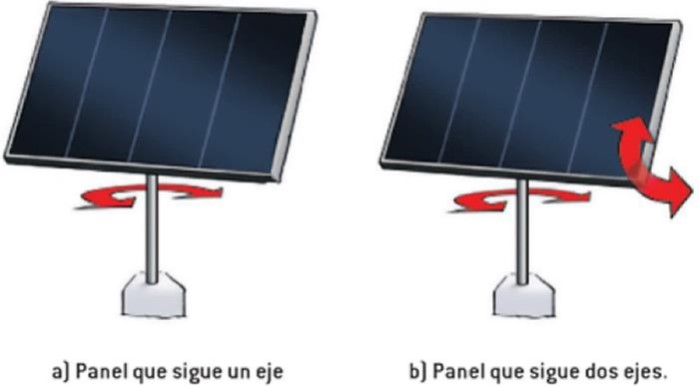
\includegraphics[width=10cm]{imagenes/panel}
	\caption{Ejes de seguimiento}
	\label{fig:paneleje}
\end{figure}

\begin{itemize}
	\item \textit{Seguidor solar en un solo eje}: Permite mover la superficie de captación sobre un solo eje, el cual puede ser horizontal, vertical u oblicuo. Tiene como ventaja que permite producir más energía eléctrica en comparación con un panel fijo. Sin embargo, no es capaz de realizar un seguimiento completo del Sol.
	\item \textit{Seguidor solar en dos ejes}: Permite mover la superficie de captación en dos ejes, lo cual brinda la capacidad de realizar un seguimiento completo del Sol. Este tipo de seguidor produce más energía que el de un solo eje, aunque suele ser más costoso.
\end{itemize}

\subsection{Robot Industrial}
De acuerdo con la Asociación de Industrias Robóticas (RIA), \textit{Un robot industrial es un manipulador multifuncional reprogramable, capaz de mover materia, piezas, herramientas o dispositivos especiales según trayectorias variables programadas para realizar tareas diversas} \cite{M6}.

\subsection{Grados de libertad}
De acuerdo con Spong en \cite{M7}, \textit{el número de GDL es igual a la dimensión del espacio de configuración. Para un robot manipulador, el número de juntas determina el número de GDL}; mientras que, según Norton en \cite{M8}, \textit{el número de GDL del sistema es igual al número de parámetros (mediciones) independientes que se requieren para definir de manera única su posición en el espacio en cualquier instante de tiempo.}

\subsection{Seguimiento solar}
Se refiere a la forma en cómo un mecanismo, sistema o dispositivo realizará el seguimiento continuo de la posición solar. Dicho seguimiento puede clasificarse en dos tipos principales:

\begin{itemize}
	\item \textit{Seguimiento activo}: Es aquel en el que el sistema retroalimenta su posicionamiento con respecto a la del Sol a través de sensores de luz. Este tipo de seguimiento permite encontrar el punto máximo de luminosidad y orientar el o los paneles solares hacia dicho punto, gracias al procesamiento y control de las señales obtenidas mediante los sensores \cite{M4}, \cite{M9}. A pesar de que es afectado por las condiciones climáticas, este seguimiento es adaptable a cualquier ubicación geográfica, siempre que sea posible detectar la luz solar.
	\item \textit{Seguimiento pasivo}: Se basa en el uso de conocimientos astronómicos y geográficos para determinar la posición solar de un determinado lugar a cualquier hora y fecha, siendo independiente de las condiciones climáticas de su entorno, por lo que no requiere de sensores o algún otro instrumento para localizar el punto más luminoso. Sin embargo, a pesar de que el seguimiento depende únicamente de las ecuaciones que predicen la posición del Sol en cualquier momento, no funcionará de la misma forma en lugares diferentes, ya que los datos geográficos cambian de un lugar a otro \cite{M4}, \cite{M9}.
\end{itemize}

\newpage
\subsection{Movimiento relativo del Sol}
La trayectoria de la Tierra alrededor del Sol es elíptica con una excentricidad alrededor de 0.0167. A la superficie que cubre esta trayectoria se le conoce como eclíptica. El eje principal de la Tierra presenta una oblicuidad respecto a la normal de la eclíptica, con un valor de $\varepsilon$=23.44°. Debido a la conservación del momento angular, el eje de rotación de la Tierra apunta en una dirección fija en el espacio a medida que la Tierra orbita alrededor del Sol. Esto significa que para la misma ubicación en la Tierra, en un momento fijo la altitud del Sol variará a lo largo del año.\\

\begin{figure}[H]
	\centering
	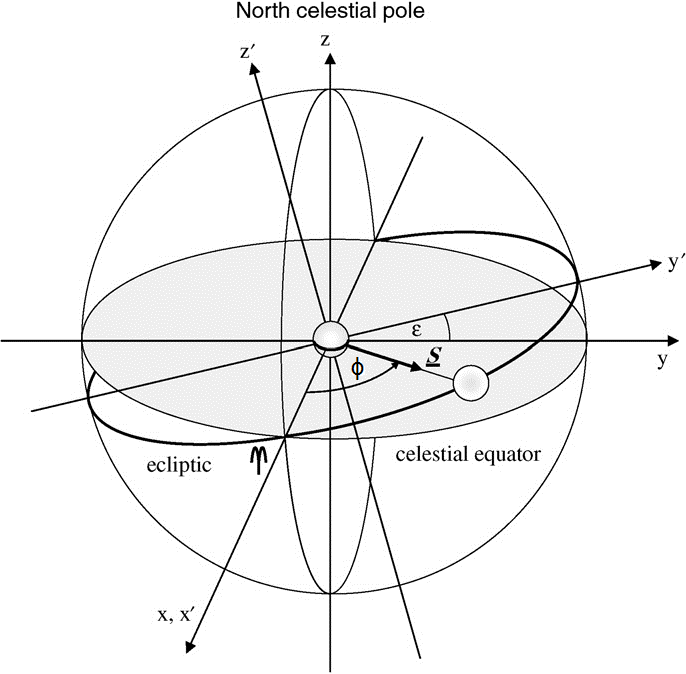
\includegraphics[width=6cm]{imagenes/ecliptica}
	\caption{Esfera celeste, que muestra la geometría del Sol y la Tierra.}
	\label{fig:ecliptica}
\end{figure}

Para el marco de referencia eclíptico, la posición del Sol se define en la Figura \ref{fig:ecliptica}, en relación con los ejes (x', y', z'), donde el origen de los ejes (x, y, z) coincide con el centro de la Tierra. El plano (x, y) (sombreado) coincide con el plano ecuatorial de la Tierra. La posición angular del Sol está definida por la longitud eclíptica $\phi$, que varía de $\phi$=0° en el equinoccio de marzo, completando 360° después de cada año. Cuando $\phi$ = 90° el Sol estará sobre la cabeza a una latitud de 23.44°N (el solsticio de junio), mientras que en el equinoccio de Septiembre $\phi$=180° y el Sol está directamente sobre la cabeza en el Ecuador. En el solsticio de diciembre $\phi$=270° y el Sol está directamente sobre la cabeza a una latitud de 23.44°S.\\

Para llevar a cabo el análisis vectorial de la geometría solar, se toma el desarrollo realizado en \cite{M10}. Con base en la Figura \ref{fig:ecliptica}, se obtiene el vector unitario S que en todo momento apunta hacia el centro del Sol con su origen en el centro geométrico de la Tierra. 

%Este vector viene dado por:\\
%
%\begin{equation}
%\vec S=cos(\phi)\hat{\imath}'+sen(\phi)\hat{\jmath}'
%\end{equation}\label{eq:sol}
%
%También se muestra en la Figura \ref{fig:ecliptica} el marco de referencia ecuatorial, que está definido por los ejes (x, y, z) donde el eje z está alineado con el eje $ N-S $ de la Tierra. El marco de referencia ecuatorial está relacionado con el marco de referencia eclíptico mediante una rotación a través de un ángulo $\varepsilon$ alrededor del eje x'. Esto refleja el hecho de que el eje $ N-S $ de la Tierra está inclinado en un ángulo $\varepsilon$ desde el plano normal al plano de la órbita aparente del Sol (es decir, el eje z').\\
%
%Al llevar a cabo la rotación, la relación entre los vectores unitarios de los 2 marcos de referencia viene dada por:
%
%\begin{equation}
%\hat{\imath}'=\hat{\imath}
%\end{equation}
%
%\begin{equation}
%\hat{\jmath}'=cos(\varepsilon)\hat{\jmath}+sen(\varepsilon)\hat{k}
%\end{equation}
%
%\begin{equation}
%\hat{k}'=-sen(\varepsilon)\hat{\jmath}+cos(\varepsilon)\hat{k}
%\end{equation}
%
%Es útil expresar el vector $ \vec S $ en términos del marco de referencia ecuatorial. Una forma de hacerlo es tomar el producto escalar del vector $ \vec S $ con los vectores unitarios ($\hat{\imath},\hat{\jmath},\hat{k}$) para determinar la magnitud de los componentes de $ \vec S $ (Sx, Sy, Sz) en (x, y, z) direcciones. Por lo tanto, en el marco de referencia ecuatorial (x, y, z), S de la ecuación \ref{eq:sol} se convierte en:

\begin{equation}\label{eq:vectorS}
\vec S = cos(\phi)\hat{\imath} + sen(\phi)cos(\varepsilon)\hat{\jmath} + sen(\phi)sen(\varepsilon)\hat{k}
\end{equation}

También se considera una referencia giratoria (x'', y'', z'') mostrada en la Figura \ref{fig:marcopolo}. Esta referencia del horizonte describe la posición del Sol desde la perspectiva de un observador en la superficie de la Tierra. La posición del Sol se describe en relación con los ejes (E, N, Z) como se muestra en la Figura \ref{fig:marcopolo}. 

%En este marco de referencia, el plano (x'', y'') todavía se encuentra en el plano ecuatorial. Sin embargo, (x'', y'', z'') es un marco de referencia giratorio de tal manera que el vector que apunta al Sol, $ \vec S $, siempre se encuentra en el plano (x'', z''). El eje z'' coincide con el eje $ N-S $ de la Tierra. 

\begin{figure}[H]
	\centering
	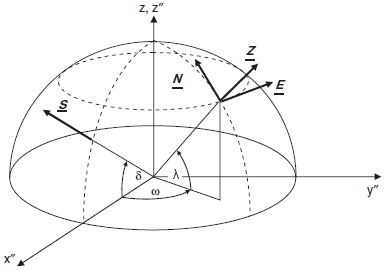
\includegraphics[width=8cm]{imagenes/marcopolo}
	\caption{Marcos de referencia giratorios ecuatoriales (x'', y'', z'') y horizontales (E, N, Z) en el hemisferio norte de la Tierra.}
	\label{fig:marcopolo}
\end{figure}

El ángulo $ \lambda $ es la latitud de la ubicación que se está considerando, $ \vec Z $ es el vector unitario normal a la horizontal del plano, $ \vec N $ es el vector unitario que apunta hacia el Polo Norte y $ \vec E $ es el vector unitario que apunta en dirección Este. $ \lambda $ se define convencionalmente como positivo en el hemisferio norte, cero en el ecuador y negativo en el hemisferio sur. En este marco de referencia, la posición angular del Sol se describe utilizando los ángulos de Elevación y Azimutal $ \alpha_s $ y $ \gamma_s $, respectivamente. Estos ángulos se muestran en la Figura \ref{fig:marcolocal}.

\begin{figure}[H]
	\centering
	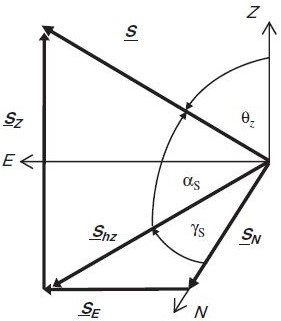
\includegraphics[width=5cm]{imagenes/marcolocal}
	\caption{Marco de referencia del horizonte para un observador posicionado en el origen de los ejes (E, N, Z), el cual está definido por el plano (E, N).}
	\label{fig:marcolocal}
\end{figure}

%\begin{equation}
%\hat E = -sen(\omega)\hat{\imath}'' + cos(\omega)\hat{\jmath}''
%\end{equation}
%
%\begin{equation}
%\hat N = -sen(\lambda)cos(\omega)\hat{\imath}'' -sen(\lambda)sen(\omega)\hat{\jmath}'' + cos(\lambda)\hat{k}''
%\end{equation}
%
%\begin{equation}
%\hat Z = cos(\lambda)cos(\omega)\hat{\imath}'' + cos(\lambda)sen(\omega)\hat{\jmath}'' + sen(\lambda)\hat{k}''
%\end{equation}
%
%\begin{equation}
%\hat S = cos(\delta)\hat{\imath}'' + sen(\delta)\hat{k}''
%\end{equation}
%
Las ecuaciones que permiten calcular las coordenadas cartesianas del Sol se obtienen al descomponer el vector descrito por la Ecuación (\ref{eq:vectorS}) en componentes colineales al marco de referencia mostrado en la Figura \ref{fig:marcolocal}. Estas expresiones se describen en las Ecuaciones (\ref{eq:Sn}), (\ref{eq:Se}) y (\ref{eq:Sz}), donde $ \delta $ es la declinación de la Tierra en función de $ \phi $ y $ \omega $ es el ángulo horario, en donde $ \omega = 0 $ se da al mediodía, $ \omega < 0 $ al amanecer y al anochecer es positivo $ \omega > 0 $. Cada 15° corresponden a 1 hora del día.
%Al realizar el producto punto entre el vector solar $ \vec S $ y las componentes del marco de referencia giratorio, se obtienen las componentes de este vector respecto a dicho marco de referencia. %
\begin{equation}\label{eq:Sn}
S_{N}=-cos(\omega)sen(\lambda)cos(\delta)+cos(\lambda)sen(\delta)
\end{equation}
\begin{equation}\label{eq:Se}
S_{E}=-sen(\omega)cos(\delta)
\end{equation}
\begin{equation}\label{eq:Sz}
S_{Z}=cos(\omega)cos(\lambda)cos(\delta)+sen(\lambda)sen(\delta)
\end{equation}
%
%\begin{equation}
%\vec S = S_{E}\bullet\hat{E}+S_{N}\bullet\hat{N}+S_{Z}\bullet\hat{Z}
%\end{equation}
%
%El vector $ \vec S $ también se puede escribir en términos de $ \alpha_s $ y $ \gamma_s $. Al analizar la Imagen \ref{fig:marcolocal}, $ \vec S $ puede escribirse como
%
%\begin{equation}
%\vec S = cos (\alpha_s) sen (\gamma_s) \bullet\hat{E} + cos (\alpha_s) cos (\gamma_s) \bullet\hat{N} + sen (\alpha_s) \bullet\hat{Z}
%\end{equation}

Con base en la Figura \ref{fig:marcolocal}, y siguiendo el desarrollo matemático de \cite{M10}, se obtienen las siguientes funciones que describen la declinación, los ángulos de Elevación y Azimutal en función del ángulo $ \phi $ y $ \omega $.

\begin{equation}\label{eq:delta}
\delta(\phi)=arcsen(sen(\phi)sen(\varepsilon))
\end{equation}
\begin{equation}\label{eq:alfa}
\alpha_s(\omega) = arcsen(cos(\omega)cos(\lambda)cos(\delta) + sen(\lambda)sen(\delta))
\end{equation}
\begin{equation}\label{eq:zeta}
\gamma_s(\omega )= arccos\left( \frac{cos(\lambda)sen(\delta) - cos(\omega)sen(\lambda)cos(\delta)}{cos(\alpha_s)}\right) 
\end{equation}

\newpage
\section{Marco procedimental}

\subsection{Sistema Mecatrónico}
Un sistema mecatrónico (SM) se define como el conjunto de dispositivos o subsistemas mecatronicos (DM) integrados sinérgicamente que buscan cumplir, realizar o resolver un objetivo o tarea compleja de forma óptima \cite{I5:2019:Online}. En la Figura \ref{fig:SM} se describe gráficamente un sistema mecatrónico.

\begin{figure}[H]
	\centering
	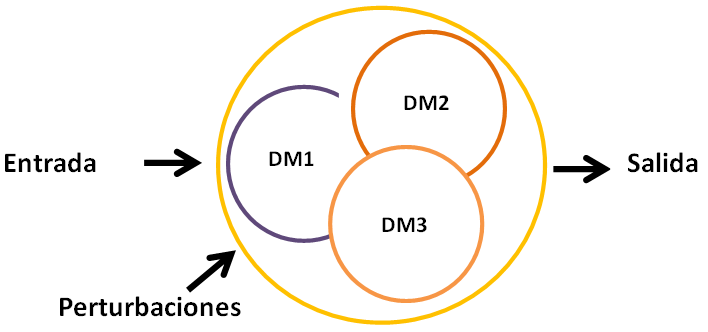
\includegraphics[width=8cm]{imagenes/SM}
	\caption{Sistema Mecatrónico}
	\label{fig:SM}
\end{figure}

El DM es capaz de interactuar con su alrededor, procesar información y generar fuerzas y movimientos específicos. En la Figura \ref{fig:DM} se aprecia un diagrama de bloques del DM.

\begin{figure}[H]
	\centering
	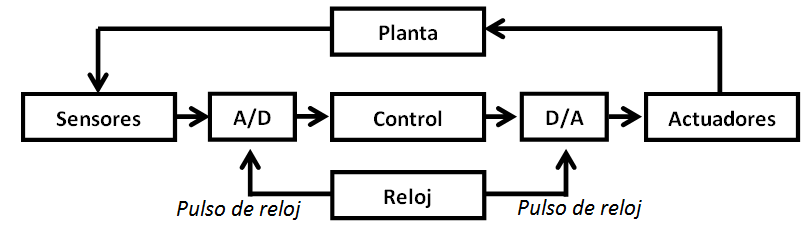
\includegraphics[width=10cm]{imagenes/DM}
	\caption{Dispositivo Mecatrónico}
	\label{fig:DM}
\end{figure}

A continuación, se describen las principales etapas del DM:
\begin{itemize}
	\item Planta: Es el proceso, máquina, dispositivo o sistema a ser controlado. 
	\item Sensores : Dispositivos que permiten detectar y/o medir magnitudes físicas o químicas. 
	\item A/D: Transforma señales analógicas en digitales, con la finalidad de que puedan ser interpretadas por la etapa de control. 
	\item Control : Parte lógica que interpreta las señales de los sensores y actúa dependiendo de la lógica programada y la información recibida. 
	\item D/A: Transformación de la señal de salida del control en la señal de entrada de los actuadores. 
	\item Actuador: Acepta un comando de control y produce un cambio en el estado físico, por la generación de fuerzas, movimientos, calor, etc. 
	\item Reloj: Se encarga de la sincronización del control. 
\end{itemize}

\subsection{Metodología de Diseño Mecatrónico}
El diseño mecatrónico es toda actividad necesaria para definir y generar soluciones a problemas específicos existentes que no se han podido resolver con anterioridad, o nuevas soluciones a problemas ya resueltos; considerando de manera concurrente y sinérgica el alcance y aplicación de cada una de las disciplinas elementales en la Mecatrónica (Mecánica, Electrónica, Control e Informática) involucradas para la solución desde las etapas iniciales en el proceso de diseño \cite{I6:2019:Online}. Para esto, se implementa una metodología de diseño mecatrónico. \\

Para este proyecto se seguirá la metodología de diseño mecatrónica basada en el modelo V, que proviene del estándar VDI 2206 para diseño de sistemas mecatrónicos \cite{M11}, \cite{M12}. Este modelo sigue una secuencia sistemática de verificación y validación a lo largo del desarrollo de todo el proyecto \cite{M13}. De acuerdo con \cite{M14}, verificación se refiere a si el sistema fue construido correctamente, mientras que validación se refiere a si se ha desarrollado el sistema correcto.\\

El modelo consiste en realizar un proceso de descomposición y definición que parte desde los requerimientos establecidos con base en las necesidades del usuario, para llegar al diseño y especificación de pequeños sistemas que cumplan los requerimientos. Posteriormente, el modelo se enfoca en las actividades de integración y validación de los sistemas, lo cual involucra el ensamble y unión de los pequeños componentes establecidos con el fin de convertirlos en sistemas más grandes que funcionen en conjunto \cite{M14}. En la Figura \ref{fig:modeloV} se muestra un esquema simplificado de este modelo.\\

\begin{figure}[H]
	\centering
	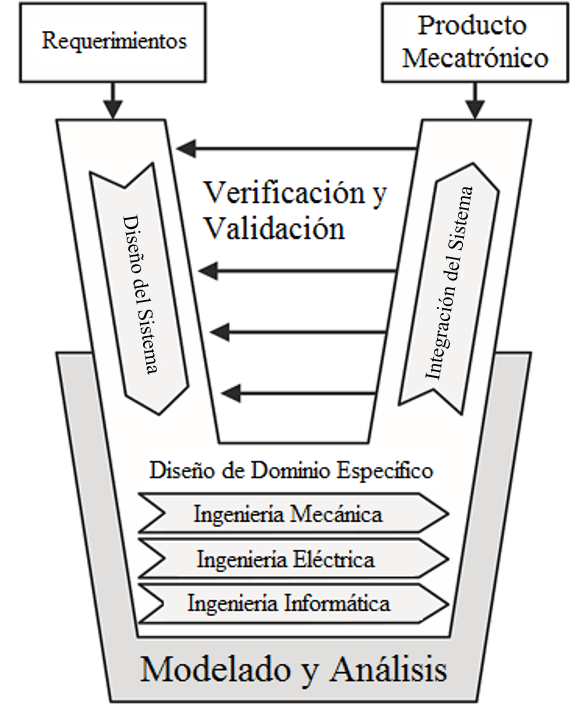
\includegraphics[width=5cm]{imagenes/modeloV}
	\caption{Esquema del modelo V \cite{I3:2013:Online}}
	\label{fig:modeloV}
\end{figure}

Con base en la metodología descrita se puede obtener una serie de fases a seguir para aplicarla al proyecto a desarrollar. Estas fases son, de forma general y tomando como referencia la descripción detallada del modelo V dada por Isermann en \cite{M13}, los siguientes:

\begin{enumerate}
	\item \textbf{Fase: Necesidades y Requerimientos.} Se indentifican las necesidades del usuario, de funcionalidad, de desempeño y demás que permitan definir lo que debe hacer el proyecto, aclarando que una necesidad puede ser el resolver un problema, lograr un objetivo o satisfacer un contrato, estándar o especificación, la cual no estará cuantificada. Estas necesidades serán posteriormente expresadas en términos técnicos y utilizadas para decisiones de diseño \cite{I1}.\\
	
	Se establecen requerimientos basándose en las necesidades identificadas, entendiendo que un requerimiento establece una condición o capacidad que debe cumplir un sistema, la cual se deriva de una necesidad de usuario, de un estándar, norma, o bien de algún documento o especificación impuesto al inicio del proceso de diseño \cite{I12}, los cuales surgirán de una transformación de las necesidades en aspectos cuantitativos y técnicos, respaldados por una previa y profunda investigación.
	
	\item \textbf{Fase: Diseño del Sistema.} Se realiza un análisis funcional, el cual permitirá describir la manera en que debe funcionar el sistema completo, así como particionar dicho sistema en funciones y subfunciones que se ajusten al cumplimiento de los requerimientos establecidos, sabiendo que una función es una transformación de una o varias entradas para producir un resultado o salida, haciendo uso de herramientas, restricciones, elementos y técnicas que permitan controlar o modificar las entradas para producir la salida deseada \cite{M14}. Se definen sistemas o módulos que cumplan con las funciones establecidas anteriormente, en los cuales ya existe la posibilidad de especificar o, al menos, proponer componentes con los que se conformarán dichos sistemas.
	
	\item \textbf{Fase: Diseño del Dominio Específico.}	Se diseñan los módulos que conformarán el proyecto a realizar, especificando distribución de tareas, componentes, software necesario, etc. Se establecen dispositivos mecatrónicos listos para ser probados e integrados.
	
	\item \textbf{Fase: Integración del Sistema.} Se integran los sistemas a nivel hardware, cubriendo aspectos de acondicionamiento, conectividad, ensambles, espacio, etc. Así mismo, se integran sistemas a nivel software, lo cual involucra aspectos de compensación, algoritmos de control, cálculo y aproximaciones, adaptabilidad, identificación y diagnóstico de fallas, por mencionar los más importantes \cite{M15}.
	
	\item \textbf{Fase: Verificación y Validación.}	La verificación consiste en determinar si cada configuración, componente y sistema cumple con los requerimientos durante la fase de diseño. Realizar pruebas, análisis, demostraciones o simulaciones, utilizando software de simulación (CAD, CAM, CAE, CAQ), modelos matemáticos, herramientas de modelado, entre otros, pueden proporcionar una verificación \cite{M14}. El proceso de verificación se enfoca en determinar si una implementación representa con precisión la descripción conceptual y los requerimientos establecidos por el o los desarrolladores del proyecto \cite{M15}. Cada requerimiento debe ser completamente verificable, de lo contrario no es un requerimiento legítimo.
	
	La validación es el proceso en el cual se determina el grado en el que una simulación equivale a una representación precisa del mundo real desde la perspectiva de los usos previstos, de acuerdo a lo definido por los requerimientos \cite{M15}. Durante la fase de diseño, la validación debe enfocarse en demostrar que el proyecto está evolucionando desde un nivel de concepto operativo, el cual refleja correctamente las necesidades y requerimientos tanto del usuario como del o los desarrolladores, así como los requerimientos a nivel sistema y componente \cite{M14}. Durante la fase de integración, la validación demuestra que el sistema que se ha diseñado e integrado cumple las necesidades y requerimientos antes identificadas y definidas por el concepto operativo \cite{M14}.
	
	Cabe mencionar que esta fase se va desarrollando de manera transversal durante la aplicación de la metodología, tanto en la fase de diseño como en la de integración.
\end{enumerate}

%\subsubsection{Necesidades y Requerimientos}
%La metodología a emplear inicia con la identificación de las necesidades del proyecto a desarrollar. En el contexto de diseño ingenieril, una necesidad puede ser el resolver un problema, lograr un objetivo o satisfacer un contrato, estándar o especificación. Cabe mencionar que una necesidad no estará cuantificada. Estas necesidades serán posteriormente expresadas en términos técnicos y utilizadas para decisiones de diseño [6].\\
%
%La metodología se enfoca principalmente en los aspectos funcionales del sistema completo, es decir, en lo que debe hacer para lograr su o sus objetivos, por lo que las necesidades identificadas deben diferenciarse entre funcionales y no funcionales, lo cual permitirá dar mayor importancia a aquellas relacionadas con la funcionalidad del proyecto. De acuerdo con Dennis M. Buede, \textit{''Una función es un proceso de transformación que cambia entradas en salidas''} [4]. Entonces, una necesidad se clasifica en funcional o no funcional dependiendo de lo que especifique; así, una \textit{necesidad funcional} describe lo que el sistema hace para lograr las expectativas del usuario, mientras que una \textit{necesidad no funcional} describe propiedades, atributos o características que el sistema debe mostrar [7]. \\
%
%A partir de las necesidades identificadas se plantean los requerimientos del proyecto, los cuales serán la base para la fase de diseño y parte de la validación.  \\
%
%A continuación, se proporciona la definición de requerimiento en el contexto de diseño ingenieril: \textit{Un requerimiento es un planteamiento o declaración que permite identificar una capacidad o función necesaria en un sistema, la cual debe satisfacer una necesidad determinada por el cliente (o el usuario)} [6].\\
%
%Se entiende entonces que un requerimiento establece una condición o capacidad que debe cumplir un sistema, la cual se deriva de una necesidad de usuario, de un estándar, norma, o bien de algún documento o especificación impuesto al inicio del proceso de diseño [8]. Es importante enfatizar que los requerimientos establecidos para el proyecto no son propuestos, sino que surgen de la transformación de las necesidades identificadas en aspectos cuantitativos, con base en una investigación exhaustiva y detallada.\\
%
%Al igual que las necesidades, los requerimientos se clasifican en funcionales y no funcionales, dependiendo de los aspectos a los que se enfoquen. Un requerimiento funcional es aquel que define las funciones que el sistema será capaz de realizar, es decir, describe las transformaciones que el sistema realiza sobre las entradas para producir salidas, enfocándose en el qué deben hacer dichas transformaciones [8]. Por otra parte, un requerimiento no funcional se relaciona con las características que de alguna forma puedan limitar al sistema, por ejemplo, el rendimiento, seguridad, fiabilidad, etc. [8] (también se les suele llamar cualidades del sistema).

%\subsubsection{Diseño del Sistema}
%La siguiente etapa consiste en el planteamiento de las funciones principales que conforman el proyecto. A partir de ellas se diseñarán los sistemas y subsistemas. \\
%
%De acuerdo con [4], una función es una transformación de una o varias entradas para producir un resultado o salida, haciendo uso de herramientas, restricciones, elementos y técnicas que permitan controlar o modificar las entradas para producir la salida deseada. Con base en lo anterior, un sistema se modela suponiendo que posee una única función de nivel superior, la cual se puede descomponer en una jerarquía de subfunciones [4]. A este proceso se le conoce como descomposición funcional, el cual comienza con la identificación de la función de más alto nivel. Dicha función se descompone en subfunciones y éstas en subfunciones más específicas; el proceso continúa hasta obtener subfunciones que realizan comportamientos o tareas específicas y que pueden implementarse con productos comerciales disponibles en el mercado [6], [9].\\
%
%La descomposición funcional descrita permite llegar a un diseño modular y mejor estructurado en comparación con otras metodologías convencionales (como el modelo en cascada), además de que muestra la secuencia lógica de las funciones y los requerimientos asociados a éstas. Sin embargo, para comprender realmente la importancia de la descomposición funcional, es necesario mostrar las relaciones existentes entre las diferentes funciones establecidas, de acuerdo a su nivel de jerarquía. Para esto se pueden emplear herramientas de modelado y análisis de sistemas. \\
%
%A grandes rasgos, la definición de los sistemas consiste en aterrizar en el dominio físico las funciones y subfunciones previamente identificadas y analizadas, ya que estas se encuentran en un dominio lógico, es decir, no son tangibles. \\
%
%El Diseño del Sistema va directamente ligado con la descomposición funcional, ya que esta última permitirá asociar funciones y subfunciones a un determinado módulo, de forma que todos los módulos planteados satisfagan las funciones antes planteadas y, por lo tanto, los requerimientos del proyecto. El objetivo será obtener posibles soluciones de dominio cruzado que partan de los módulos identificados, las cuales describan las características físicas y lógicas esenciales del proyecto [1].\\
%
%Una vez que se tienen las posibles soluciones y se han considerado los aspectos ya mencionados de un sistema mecatrónico, se procederá a seleccionar la solución final sobre la cual se llevará a cabo el diseño de los módulos. Dicho diseño deberá comprender los aspectos técnico, funcional y tecnológico [10], haciendo uso de herramientas de selección, simulaciones, modelado y cálculo. Todo lo anterior deberá garantizar el correcto desempeño funcional y el cumplimiento de los requerimientos identificados [1]. 

%\subsubsection{Integración del Sistema}
%Al definir los módulos o sistemas que se diseñarán, deben considerarse ciertos atributos clave de cualquier sistema mecatrónico, los cuales se basan en la integración funcional y espacial de subsistemas mecánicos, eléctricos y de procesamiento de información. Además, debido al hecho de que un sistema mecatrónico solo puede completar sus tareas exitosamente si todos sus elementos funcionan en armonía (o de forma sinérgica), en este nivel de diseño será necesaria la combinación de conocimientos tanto teóricos como físicos y tecnológicos de diferentes dominios científicos y de ingeniería para el diseño del o los sistemas (o módulos) propuestos [10].

%\subsubsection{Verificación y validación}
%Como se mencionó antes, se debe asegurar que los módulos o sistemas desarrollados cumplan con los requerimientos establecidos anteriormente, por lo que la solución propuesta debe compararse con los requerimientos a lo largo de la metodología seguida, proceso al cual se le llama verificación y validación [11]. \\
%
%La verificación consiste en determinar si cada configuración, componente y sistema cumple con los requerimientos durante la fase de diseño. Realizar pruebas, análisis, demostraciones o simulaciones puede proporcionar una verificación [4]. El proceso de verificación se enfoca en determinar si una implementación representa con precisión la descripción conceptual y los requerimientos establecidos por el o los desarrolladores del proyecto [10]. Cada requerimiento debe ser completamente verificable, de lo contrario no es un requerimiento legítimo.\\
%
%La validación es el proceso en el cual se determina el grado en el que una simulación equivale a una representación precisa del mundo real desde la perspectiva de los usos previstos, de acuerdo a lo definido por los requerimientos [10]. Durante la fase de diseño, la validación debe enfocarse en demostrar que el proyecto está evolucionando desde un nivel de concepto operativo, el cual refleja correctamente las necesidades y requerimientos tanto del usuario como del o los desarrolladores, así como los requerimientos a nivel sistema y componente [4]. Durante la fase de integración, la validación demuestra que el sistema que se ha diseñado e integrado cumple las necesidades y requerimientos antes identificadas y definidas por el concepto operativo [4].

\subsection{Herramientas de diseño}
\subsubsection{\textit{Integration Definition for Function Modeling} (IDEF0)}
Es una técnica de modelado para el análisis, desarrollo e integración de sistemas, la cual muestra el flujo de datos, el control de sistemas y el flujo funcional. Esta técnica consiste en una serie de diagramas, textos y términos interrelacionados de forma jerárquica \cite{I5:2019:Online}. Su proceso comienza con la identificación de la función primordial a ser descompuesta. Conforme avanza el proceso de descomposición, se van introduciendo más y más niveles de detalle a través de la estructura del modelo \cite{I6:2019:Online}. 

Un modelo IDEF0 se conforma de dos o más páginas IDEF0. Una página IDEF0 posee dos elementos básicos, funciones y flujo de información, energía o materia. Por razones de legibilidad, cada página debe limitarse a un máximo de 6 o 7 subfunciones \cite{M14}. Dichas subfunciones suelen colocarse en forma diagonal descendente, siguiendo una especie de jerarquía enfocada a qué función tiene más importancia en la entrada y cuál en la salida.

Una función se representa por una caja o recuadro descrita por una frase verbo-sustantivo y es numerada para su identificación dentro del contexto del modelo \cite{M14}. Cada función posee entradas y salidas; las entradas a ser transformadas en salidas llegan por la izquierda, los controles que guían el proceso de transformación llegan por arriba, los mecanismos y recursos físicos llegan por debajo, y las salidas parten de la derecha \cite{I5:2019:Online}, tal y como se muestra en la Figura \ref{fig:idef0b}. Es importante mencionar que, si bien las entradas son opcionales, los controles siempre deben estar presentes.
\begin{figure}[H]
	\centering
	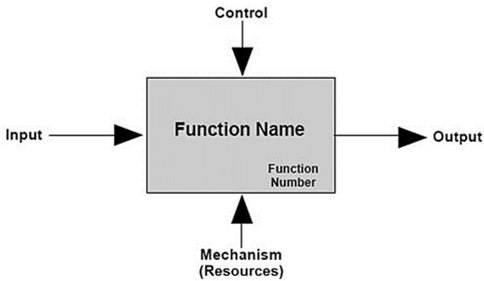
\includegraphics{imagenes/idef0b}
	\caption{Formato de recuadro IDEF0 \cite{I5:2019:Online}.}
	\label{fig:idef0b}
\end{figure}

\subsubsection{Análisis morfológico}
Es un método para la investigación de características asociadas a un problema complejo no cuantificables, las cuales contienen un sin fin de parámetros. Es de gran ayuda para la delimitación de un proyecto y también es útil para examinar y analizar diversas combinaciones de configuraciones y obtener así posibles soluciones al problema \cite{M16}.

Para emplear esta herramienta, el problema debe estar bien definido y se debe considerar que cualquier parámetro puede ser importante para el análisis. Entonces, se construye una matriz multidimensional que contiene todas las posibles soluciones del problema a resolver \cite{M16}. La solución final elegida debe apoyarse en métodos que complementen esta herramienta, por lo que el análisis morfológico en sí no es suficiente para generar la solución final.
La matriz consiste de renglones y columnas, así cada celda contiene un valor particular o condición por cada parámetro. Los renglones contienen los parámetros o características a tomar en cuenta, las cuales deben ser funcionales preferentemente. Las columnas contienen las diversas soluciones que pudieran satisfacer cada característica del problema.

Es importante recalcar que esta no es una herramienta de selección y que al emplearla no deben incluirse materiales, componentes ni lenguajes de programación \cite{M17}, ya que, como su nombre lo dice, todas las soluciones deben ir asociadas a formas y geometrías.

\subsubsection{\textit{Analytic Hierarchy Process} (AHP)}
Es una herramienta de selección multicriterio, la cual permite descomponer estructuras complejas en componentes, los cuales se ordenan de forma jerárquica y se les asignan valores numéricos para ser evaluados y así determinar qué componente tiene alta prioridad \cite{I17}. En la Figura \ref{fig:AHP1} se muestra un esquema de esta red estructurada jerárquicamente.\\

\begin{figure}[H]
	\centering
	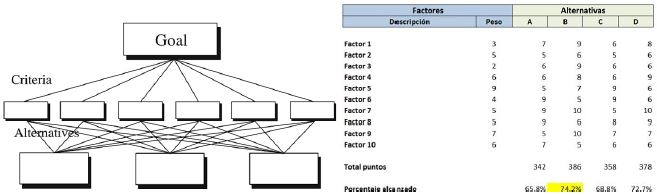
\includegraphics[width=\columnwidth]{imagenes/RedAHP}
	\caption{Red AHP de 3 niveles de jerarquía (izquierda) \cite{I17} y matriz ponderada (derecha).}
	\label{fig:AHP1}
\end{figure}

Una de las grandes ventajas de esta herramienta es que permite un refinamiento bastante flexible en la intensidad de importancia para cada elemento, con lo cual es capaz de indicar qué tan superior es un elemento con respecto a otro en grados que pueden ir desde muy ligeramente, moderadamente hasta fuertemente superior.

La tarea de establecer prioridades requiere que los criterios, subcriterios, propiedades o características de las alternativas se comparen entre sí. Los juicios de comparación se aplican a elementos homogéneos, con base en una escala fundamental de valores que representa las intensidades de los juicios \cite{M18}. Esta escala (si bien se compone de 9 puntos, nosotros solo tomaremos 5) se muestra en la Tabla \ref{tabla:AHP}.

\begin{table}[H]
	\centering
	\caption{Escala fundamental del método AHP \cite{I9}}
	\begin{tabular}{@{}|p{2.5cm}|p{5cm}|p{5.5cm}|} 
		\hline
		\textbf{Intensidad de importancia} & \textbf{Definición} & \textbf{Explicación}  \\
		\hline \hline
		1 & Igual importancia & Dos actividades contribuyen igualmente al objetivo\\ \hline
		2 & Débil &  \\ \hline
		3 & Importancia moderada & Experiencia y juicio ligeramente a favor de una actividad sobre otra\\ \hline
		4 & Moderado plus &  \\ \hline
		5 & Gran importancia & Experiencia y juicio fuertemente a favor de una actividad sobre otra\\ \hline
		Recíprocos de arriba & Si la actividad \textit{i} tiene uno de los números distintos de cero asignado a ella cuando se compara con la actividad \textit{j}, entonces \textit{j} tiene el valor recíproco cuando se compara con \textit{i} & Una razonable suposición\\ \hline
		
	\end{tabular}	
	\label{tabla:AHP}
\end{table}

\subsubsection{Árbol de decisiones}
Es un mapa de los posibles resultados de una serie de decisiones relacionadas. Permite que un individuo o una organización comparen posibles acciones entre sí según sus costos, probabilidades y beneficios. Con el objetivo de filtrar el gran número de componentes que puedan requerirse, se utilizan estos árboles de decisión, por medio de preguntas rápidas que permitirán eliminar opciones sin necesidad de aplicar el método de selección multicriterio para todas estas, reduciendo la complejidad de operaciones y minimizando el tiempo necesario para la selección.

Un árbol de decisiones, por lo general, comienza con un único nodo y se ramifica en resultados posibles. Cada resultado puede crear nodos adicionales, que se ramifican en otras posibilidades. Un ejemplo de este se puede ver en la Figura \ref{fig:arbol}.

Hay 3 tipos diferentes de nodos: de probabilidad, de decisión y nodos terminales. Un nodo de probabilidad (representado con un círculo) muestra las probabilidades de ciertos resultados. Un nodo de decisión (representado con un cuadrado) muestra una decisión que se tomará, y un nodo terminal muestra el resultado definitivo de una ruta de decisión. A continuación, se explica cómo debe realizarse el trazo de un árbol de decisión.

\begin{enumerate}
	\item \textbf{Comenzar con la decisión principal.}
	Dibujar un pequeño cuadro, luego dibujar una línea desde el recuadro hacia la derecha para cada posible solución o acción.
	\item \textbf{Agregar nodos de decisión y probabilidad} para expandir el árbol:
	\begin{itemize}
		\item Si otra decisión es necesaria, dibujar otro recuadro.
		\item Si el resultado es incierto, dibujar un círculo.
		\item Si el problema está resuelto, dejarlo en blanco (por el momento).
	\end{itemize}
	Desde cada nodo de decisión dibujar soluciones posibles. Desde cada nodo de probabilidad dibujar líneas que representen los resultados posibles. Si se desea analizar opciones de forma numérica, incluir la probabilidad de cada resultado y el costo de cada acción.
	\item \textbf{Continuar con la expansión hasta que cada línea alcance un extremo}, lo que significa que no hay más decisiones o resultados que considerar. Luego, asignar un valor a cada resultado posible. Agregar triángulos para indicar los extremos.
\end{enumerate}

\begin{figure}[H]
	\centering
	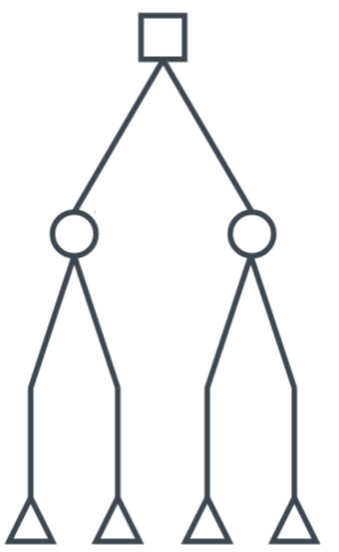
\includegraphics[width=3cm]{imagenes/arbol}
	\caption{Ejemplo de árbol de decisiones}
	\label{fig:arbol}
\end{figure}
%%%%%%fin del archivo
\endinput